\documentclass[a4paper, titlepage]{article}
\usepackage{hyperref}
\usepackage[section]{algorithm}
\usepackage[numbered]{algo}
\usepackage[left=1cm,right=1.5cm,top=1cm,bottom=2cm]{geometry}
\linespread{1.5}
\usepackage{amsmath,scalerel}
\usepackage{pgfplots}
\pgfplotsset{compat=1.18}
\usepackage{graphicx}
\usepackage{xepersian}
\settextfont[Scale=1.2]{B-NAZANIN.TTF}
\usepackage{indentfirst}
\usetikzlibrary{arrows}

\graphicspath{ {./img/} }

\title{
    \center
    \includegraphics[height=5cm]{logo.jpg} \\
    دانشکده مهندسی کامپیوتر \\[25pt]     
    ارائه یادگیری ماشین
}

\author{
     بهنود قربانی - علیرضا لیمویی - امیررضا ارجمند
}

\date{}

\begin{document}

\maketitle
\tableofcontents


\section{مقدمه}

\subsection{تعریف یادگیری ماشین}
\subsubsection{یادگیری ماشین چیست؟}

یادگیری ماشین شاخه‌ای از هوش مصنوعی (\lr{AI}) است که بر ساخت سیستم‌هایی تمرکز دارد که قادر به یادگیری و تصمیم‌گیری بر اساس داده‌ها هستند. برخلاف برنامه‌نویسی سنتی که در آن توسعه‌دهنده دستورات صریحی برای سیستم می‌نویسد، یادگیری ماشین شامل ایجاد الگوریتم‌هایی است که به سیستم اجازه می‌دهد الگوها را شناسایی کند، پیش‌بینی کند و با تجربه بهبود یابد.

\subsubsection{مفاهیم کلیدی یادگیری ماشین}

الگوریتم‌ها: هسته یادگیری ماشین، الگوریتم‌ها مدل‌های ریاضی هستند که داده‌ها را پردازش کرده و از آن‌ها یاد می‌گیرند. الگوریتم‌های رایج شامل رگرسیون خطی، درخت‌های تصمیم‌گیری و شبکه‌های عصبی هستند.

داده‌ها: سوخت یادگیری ماشین. می‌تواند ساختاریافته (مثل پایگاه‌های داده و صفحات گسترده) یا غیرساختاریافته (مثل متن، تصاویر و ویدیوها) باشد. کیفیت و کمیت داده‌ها به شدت بر عملکرد مدل تأثیر می‌گذارد.

آموزش: فرآیند وارد کردن داده‌ها به الگوریتم یادگیری ماشین برای کمک به یادگیری آن. در طول آموزش، الگوریتم پارامترهای خود را تنظیم می‌کند تا خطاها را به حداقل برساند.

آزمون: پس از آموزش، مدل با داده‌های جدید آزمایش می‌شود تا دقت و عملکرد آن ارزیابی شود. این کمک می‌کند تا مشخص شود مدل چقدر به داده‌های نادیده تعمیم می‌دهد.
\subsection{هوش مصنوعی و طبیعی}
\subsubsection{تفاوت بین هوش مصنوعی و هوش طبیعی}

هوش مصنوعی (\lr{AI}) و هوش طبیعی (\lr{NI}) هر دو به توانایی یادگیری و حل مسائل اشاره دارند، اما با تفاوت‌های بنیادینی در نحوه عملکرد و مکانیسم‌های زیرساختی همراه هستند:

هوش مصنوعی (\lr{AI})
منشأ: توسط انسان‌ها ساخته و برنامه‌ریزی می‌شود.

ساختار: بر پایه الگوریتم‌ها و مدل‌های ریاضی استوار است.

یادگیری: از طریق پردازش حجم وسیعی از داده‌ها و استفاده از تکنیک‌های یادگیری ماشین.

انطباق‌پذیری: توانایی انطباق با شرایط جدید و به‌روز‌رسانی مدل‌ها براساس داده‌های جدید.

محدودیت‌ها: در محدوده داده‌های ورودی و طراحی الگوریتم‌ها عمل می‌کند؛ فاقد خلاقیت و درک واقعی است.

هدف: انجام وظایف خاص و حل مسائل مشخص.

هوش طبیعی (\lr{NI})
منشأ: در موجودات زنده، به‌ویژه انسان‌ها، ذاتی است.

ساختار: بر پایه مغز و سیستم عصبی استوار است.

یادگیری: از طریق تجربه، آموزش، تعاملات اجتماعی و فرآیندهای شناختی.

انطباق‌پذیری: بسیار انعطاف‌پذیر، قادر به یادگیری و تطبیق در محیط‌های متغیر و نامشخص.

محدودیت‌ها: محدود به توانایی‌های فیزیکی و روانی انسان‌ها؛ ممکن است با خطا و تعصب همراه باشد.

هدف: بقا، تطبیق با محیط، خلاقیت و درک عمیق از جهان.

\subsubsection{نحوه یادگیری انسان‌ها در مقابل \lr{AI}}


یادگیری انسان‌ها

تجربه مستقیم: انسان‌ها از طریق تجربه‌های شخصی و تعاملات با محیط یاد می‌گیرند.
مشاهده و تقلید: یادگیری از طریق مشاهده رفتارهای دیگران و تقلید آن‌ها.
آموزش رسمی: از طریق آموزش‌های ساختاریافته مانند مدارس و دانشگاه‌ها.
تکرار و تمرین: تمرین مداوم مهارت‌ها تا تسلط بر آن‌ها.
انعکاس و تفکر: توانایی تأمل و ارزیابی تجربیات گذشته برای بهبود یادگیری.
احساسات و انگیزه‌ها: نقش مهمی در فرآیند یادگیری دارند، به عنوان مثال، علاقه و انگیزه می‌توانند یادگیری را تسریع کنند.


یادگیری\lr{AI}

داده‌های برچسب‌دار: مدل‌های \lr{AI} از طریق داده‌های برچسب‌دار (\lr{supervised learning}) آموزش می‌بینند، که به آن‌ها کمک می‌کند الگوها و روابط را شناسایی کنند.
الگوریتم‌ها: استفاده از الگوریتم‌های یادگیری ماشین مانند رگرسیون، درخت‌های تصمیم، و شبکه‌های عصبی.
بازخورد: مدل‌های \lr{AI} از طریق بازخورد اصلاح می‌شوند؛ مثلاً الگوریتم‌های یادگیری تقویتی از طریق پاداش و جریمه بهبود می‌یابند.
تکرار و به‌روزرسانی: مدل‌ها با داده‌های جدید به‌روزرسانی و مجدداً آموزش داده می‌شوند تا دقت و کارایی آن‌ها افزایش یابد.
پردازش موازی: استفاده از قدرت محاسباتی بالا برای پردازش حجم وسیعی از داده‌ها به طور همزمان.
\subsection{الگوریتم های یادگیری ماشین}
\subsubsection{\lr{Supervised learning}}

یادگیری نظارت‌شده چیست؟

یادگیری نظارت‌شده (\lr{Supervised Learning}) یکی از روش‌های یادگیری ماشین است که در آن مدل با استفاده از داده‌های برچسب‌دار آموزش داده می‌شود. این به این معناست که هر ورودی در مجموعه داده‌ها با خروجی صحیح (برچسب) مرتبط است. هدف از یادگیری نظارت‌شده این است که مدل بتواند با دیدن داده‌های جدید و نامعلوم، خروجی‌های صحیح را پیش‌بینی کند.

مراحل یادگیری نظارت‌شده

جمع‌آوری داده‌ها: جمع‌آوری مجموعه‌ای از داده‌های ورودی و خروجی‌های مرتبط با آن‌ها. این داده‌ها به عنوان داده‌های آموزشی استفاده می‌شوند
.
تقسیم داده‌ها: تقسیم داده‌ها به دو مجموعه: داده‌های آموزشی (\lr{training data}) و داده‌های آزمون(\lr{test data}).

انتخاب مدل: انتخاب الگوریتم مناسب برای یادگیری. مثال‌هایی از الگوریتم‌ها عبارتند از رگرسیون خطی، درخت تصمیم‌گیری، ماشین بردار پشتیبان (\lr{SVM})، و شبکه‌های عصبی.
آموزش مدل: تغذیه داده‌های آموزشی به مدل و تنظیم پارامترهای آن به گونه‌ای که خطا بین خروجی پیش‌بینی شده و خروجی واقعی به حداقل برسد.

ارزیابی مدل: استفاده از داده‌های آزمون برای ارزیابی عملکرد مدل و اطمینان از این که مدل به خوبی تعمیم یافته است.

استفاده از مدل: استفاده از مدل آموزش دیده برای پیش‌بینی خروجی‌های داده‌های جدید و نامعلوم.

\subsubsection{\lr{Unsupervised learning}}

یادگیری بدون نظارت چیست؟

یادگیری بدون نظارت (\lr{Unsupervised Learning}) یکی از روش‌های یادگیری ماشین است که در آن مدل بدون استفاده از داده‌های برچسب‌دار آموزش داده می‌شود. در یادگیری بدون نظارت، داده‌ها تنها شامل ورودی‌ها هستند و خروجی‌های مشخصی به مدل داده نمی‌شود. هدف از این نوع یادگیری کشف الگوها، ساختارها یا ویژگی‌های مهم در داده‌ها است.

مراحل یادگیری بدون نظارت

جمع‌آوری داده‌ها: جمع‌آوری مجموعه‌ای از داده‌های ورودی بدون برچسب
.
انتخاب مدل: انتخاب الگوریتم مناسب برای یادگیری. مثال‌هایی از الگوریتم‌ها عبارتند از خوشه‌بندی (\lr{clustering}) و کاهش ابعاد (\lr{dimensionality reduction}).

آموزش مدل: تغذیه داده‌ها به مدل و استفاده از الگوریتم‌های یادگیری بدون نظارت برای شناسایی الگوها و ساختارها.

تفسیر نتایج: تفسیر و تحلیل نتایج به دست آمده برای استخراج دانش مفید از داده‌ها.

استفاده از مدل: استفاده از مدل آموزش دیده برای اعمال به داده‌های جدید و شناسایی الگوهای مشابه.

\subsubsection{\lr{Reinforcement learning}}

یادگیری تقویتی چیست؟

یادگیری تقویتی (\lr{Reinforcement Learning}) یکی از روش‌های یادگیری ماشین است که در آن یک عامل (\lr{Agent}) از طریق تعامل با محیط، یاد می‌گیرد که چگونه با انجام یک سری از اعمال (\lr{Actions}) در موقعیت‌های مختلف (\lr{States}) بیشترین پاداش (\lr{Reward}) ممکن را دریافت کند. هدف یادگیری تقویتی یافتن سیاست بهینه (\lr{Optimal Policy}) است که حداکثر پاداش بلندمدت را تضمین می‌کند.

عناصر کلیدی یادگیری تقویتی

عامل (\lr{Agent}): موجودیتی که تصمیم‌گیری می‌کند و اعمال را انجام می‌دهد.

محیط (\lr{Environment}): جایی که عامل در آن عمل می‌کند و از آن پاداش و بازخورد دریافت می‌کند.

وضعیت‌ها (\lr{States}): نمایشگر وضعیت فعلی محیط.

اعمال (\lr{Actions}): مجموعه‌ای از اقدامات که عامل می‌تواند انجام دهد.

پاداش (\lr{Reward}): بازخوردی که عامل پس از انجام یک عمل دریافت می‌کند. پاداش می‌تواند مثبت یا منفی باشد.

سیاست (\lr{Policy}): استراتژی‌ای که عامل برای انتخاب اعمال بر اساس وضعیت‌ها استفاده می‌کند.

تابع ارزش (\lr{Value Function}): تخمین ارزش بلندمدت وضعیت‌ها یا وضعیت-عمل‌ها.

مراحل یادگیری تقویتی

آغاز وضعیت: عامل در یک وضعیت اولیه شروع می‌کند.

انتخاب عمل: عامل بر اساس سیاست فعلی یک عمل را انتخاب می‌کند.

اجرای عمل و دریافت پاداش: عامل عمل را اجرا کرده و پاداش فوری را دریافت می‌کند. همچنین وضعیت جدید را مشاهده می‌کند.

به‌روزرسانی سیاست: عامل سیاست خود را بر اساس تجربه جدید به‌روزرسانی می‌کند تا پاداش بلندمدت خود را بهبود بخشد.

تکرار: مراحل فوق تا زمانی تکرار می‌شوند که سیاست بهینه یافت شود یا زمان معین شده پایان یابد.

\subsection{یادگیری ماشین چگونه اتفاق می افتد}
مثال "ربات سازنده" و "ربات معلم
"

سناریو

فرض کنید که ما دو ربات داریم: ربات سازنده (\lr{Builder Bot}) و ربات معلم (\lr{Teacher Bot}). هدف این است که ربات سازنده یاد بگیرد چگونه سازه‌های مختلفی را با استفاده از قطعات ساختمانی بسازد. ربات معلم نقش مربی را ایفا می‌کند و داده‌های آموزشی را برای ربات سازنده فراهم می‌کند.

مراحل انجام کار

جمع‌آوری داده‌ها توسط ربات معلم:

ربات معلم یک سری سازه‌های کامل شده با قطعات ساختمانی دارد.
برای هر سازه، یک مجموعه از قطعات (ورودی‌ها) و ترتیب ساخت (برچسب‌ها) موجود است.
داده‌های آموزشی شامل مجموعه‌های قطعات به همراه ترتیب صحیح ساخت آن‌ها می‌شود.

تقسیم داده‌ها:

داده‌های جمع‌آوری شده به دو قسمت تقسیم می‌شوند: داده‌های آموزشی برای آموزش ربات سازنده و داده‌های آزمون برای ارزیابی عملکرد آن.

انتخاب مدل:

یک مدل یادگیری نظارت‌شده، مثل شبکه عصبی یا درخت تصمیم‌گیری، برای آموزش انتخاب می‌شود.

آموزش مدل:

ربات سازنده داده‌های آموزشی را از ربات معلم دریافت می‌کند.
مدل یادگیری با استفاده از این داده‌ها آموزش داده می‌شود تا الگوها و ترتیب‌های صحیح ساخت سازه‌ها را بیاموزد.

ارزیابی مدل:

ربات سازنده مدل آموزش دیده را با داده‌های آزمون ارزیابی می‌کند تا عملکرد آن را بسنجد.
دقت مدل در پیش‌بینی ترتیب صحیح ساخت سازه‌ها بررسی می‌شود.
استفاده از مدل:

ربات سازنده حالا می‌تواند با استفاده از مدل آموزش دیده، سازه‌های جدیدی را با ترتیب صحیح بسازد.
ربات سازنده قادر است با دریافت مجموعه‌ای از قطعات، ترتیب صحیح ساخت را پیش‌بینی کرده و سازه مورد نظر را بسازد.
مثال عددی

فرض کنید داده‌های آموزشی شامل 10 نوع سازه مختلف است که هر کدام از آن‌ها با قطعات مختلفی ساخته شده‌اند. به عنوان مثال:

سازه 1: قطعات\lr{A}، \lr{B}، \lr{C} (ترتیب ساخت: \lr{A} \lr{→} \lr{B} \lr{→} \lr{C})

سازه 2: قطعات \lr{D}، \lr{E}، \lr{F} (ترتیب ساخت: \lr{D} \lr{→} \lr{E} \lr{→} \lr{F})

ربات معلم این داده‌ها را به ربات سازنده می‌دهد. ربات سازنده مدل خود را با استفاده از این داده‌ها آموزش می‌دهد. سپس، ربات سازنده با دریافت مجموعه‌ای از قطعات جدید (مثلاً \lr{G}، \lr{H}، \lr{I}) قادر خواهد بود ترتیب صحیح ساخت (مثلاً \lr{G} \lr{→} \lr{H} \lr{→} \lr{I}) را پیش‌بینی کند و سازه را بسازد.


\begin{figure}
    \centering
    \includegraphics[width=0.5\linewidth]{Builder robot and teacher robot.PNG}
    \caption{\lr{Builder robot and Teacher robot}}
    \label{Builder robot and Teacher robot}
\end{figure}



خلاصه
\label
ساختار: استفاده از منطق، قواعد و الگوریتم‌های قطعی (\lr{Deterministic}).

منطق: بر پایه برنامه‌نویسی صریح و تعریف قواعد دستوری است.

مثال‌ها: سیستم‌های خبره (\lr{Expert Systems})، موتورهای قانون‌گذاری (\lr{Rule Engines})، منطق فازی (\lr{Fuzzy Logic}).

قابلیت یادگیری: به طور کلی، سیستم‌های هوش مصنوعی کلاسیک توانایی یادگیری از داده‌ها را ندارند و بر اساس قواعد از پیش تعیین‌شده عمل می‌کنند.

کاربردها: اتوماسیون فرآیندها، سیستم‌های تشخیص خطا، بازی‌های شطرنج اولیه، سیستم‌های توصیه‌گر ساده.

2. یادگیری ماشین (\lr{Machine Learning})
یادگیری ماشین زیرمجموعه‌ای از هوش مصنوعی است که در آن سیستم‌ها از طریق داده‌ها و تجربیات یاد می‌گیرند و بهبود می‌یابند.

ساختار: استفاده از الگوریتم‌ها و مدل‌های آماری برای تحلیل و یادگیری از داده‌ها.

منطق: بر پایه الگوهای موجود در داده‌ها و تجربه‌های گذشته است.

مثال‌ها: رگرسیون خطی و لجستیک، درخت‌های تصمیم‌گیری، شبکه‌های عصبی، ماشین‌های بردار پشتیبان (\lr{SVM}).

قابلیت یادگیری: سیستم‌های یادگیری ماشین با استفاده از داده‌ها آموزش می‌بینند و توانایی بهبود و تطبیق با داده‌های جدید را دارند.

کاربردها: تشخیص تصویر و صدا، پردازش زبان طبیعی، توصیه‌گرهای پیچیده، سیستم‌های پیش‌بینی، خودروهای خودران.

تفاوت‌های کلیدی

1. روش‌های حل مسئله

هوش مصنوعی کلاسیک: مشکلات را با استفاده از قواعد و منطق صریح حل می‌کند. به عنوان مثال، یک سیستم خبره پزشکی ممکن است بر اساس مجموعه‌ای از قواعد از پیش تعریف‌شده برای تشخیص بیماری‌ها عمل کند.

یادگیری ماشین: مشکلات را با استفاده از الگوهای موجود در داده‌ها حل می‌کند. به عنوان مثال، یک مدل یادگیری ماشین می‌تواند با تحلیل داده‌های پزشکی، الگوهایی را شناسایی کرده و پیش‌بینی‌هایی درباره بیماری‌ها انجام دهد.

2. انعطاف‌پذیری و تطبیق‌پذیری

هوش مصنوعی کلاسیک: انعطاف‌پذیری کمتری دارد زیرا بر اساس قواعد سخت‌گیرانه‌ای که از پیش تعریف شده‌اند عمل می‌کند.

یادگیری ماشین: انعطاف‌پذیری بیشتری دارد زیرا می‌تواند از داده‌های جدید یاد بگیرد و خود را با تغییرات تطبیق دهد.

3. نیاز به داده‌ها

هوش مصنوعی کلاسیک: به داده‌های برچسب‌دار و زیادی نیاز ندارد زیرا بر اساس قواعد ثابت عمل می‌کند.

یادگیری ماشین: به داده‌های برچسب‌دار و حجیم نیاز دارد تا بتواند الگوها را شناسایی کند و مدل‌های دقیقی بسازد.

4. عملکرد در شرایط نامعین

هوش مصنوعی کلاسیک: عملکرد ضعیفی در شرایط نامعین و پیچیده دارد زیرا به قواعد از پیش تعریف‌شده وابسته است.

یادگیری ماشین: عملکرد بهتری در شرایط نامعین و پیچیده دارد زیرا می‌تواند از داده‌ها یاد بگیرد و خود را تطبیق دهد.

\subsection{مدل یادگیری ماشین چیست}

یک مدل یادگیری ماشین یک نمایش ریاضی یا الگوریتم است که برای یادگیری الگوها از داده‌ها و انجام پیش‌بینی‌ها یا تصمیم‌گیری‌ها بر اساس داده‌های جدید طراحی شده است. این مدل از طریق فرآیندی به نام آموزش ساخته می‌شود که در آن مدل با داده‌های تاریخی مواجه شده و توانایی شناسایی روابط و الگوها را پیدا می‌کند.

اجزای اصلی یک مدل یادگیری ماشین:

داده‌ها:

داده‌های آموزشی: برای آموزش مدل استفاده می‌شود و شامل ویژگی‌های ورودی و برچسب‌های خروجی متناظر است.

داده‌های اعتبارسنجی: برای تنظیم ابرپارامترهای مدل و جلوگیری از بیش‌برازش استفاده می‌شود.

داده‌های آزمایشی: برای ارزیابی عملکرد مدل بر روی داده‌های نادیده استفاده می‌شود.

ویژگی‌ها: متغیرها یا ورودی‌هایی که برای انجام پیش‌بینی‌ها استفاده می‌شوند. ویژگی‌ها معمولاً عددی هستند، اما می‌توانند شامل داده‌های دسته‌ای نیز باشند.

برچسب‌ها/اهداف: خروجی‌ها یا نتایجی که مدل قصد دارد پیش‌بینی کند.

انواع مدل‌های یادگیری ماشین:

رگرسیون خطی: نتایج پیوسته را بر اساس روابط خطی بین ویژگی‌ها و هدف پیش‌بینی می‌کند.

رگرسیون لجستیک: نتایج باینری را با استفاده از یک تابع لجستیک پیش‌بینی می‌کند.

درخت‌های تصمیم‌گیری: از یک مدل درخت‌مانند برای وظایف طبقه‌بندی یا رگرسیون استفاده می‌کند.

\begin{figure}
    \centering
    \includegraphics[width=0.5\linewidth]{image_2024-05-27_20-39-48.png}
    \caption{\lr{Desicion tree}}
    \label{Desicion tree}
\end{figure}

جنگل تصادفی: مجموعه‌ای از درخت‌های تصمیم‌گیری برای بهبود دقت و کاهش بیش‌برازش.

ماشین‌های بردار پشتیبان (\lr{SVM}): صفحه فوق بهینه را برای جدا کردن دسته‌های مختلف پیدا می‌کند.

شبکه‌های عصبی: متشکل از لایه‌هایی از گره‌های متصل (نورون‌ها) که الگوهای پیچیده را یاد می‌گیرند.

خوشه‌بندی \lr{K}-میانگین: یک روش بدون نظارت برای تقسیم‌بندی داده‌ها به خوشه‌ها بر اساس شباهت.

تحلیل مؤلفه‌های اصلی (\lr{PCA}): تکنیکی برای کاهش ابعاد داده‌ها در حالی که اکثر واریانس را حفظ می‌کند.

\subsection{کاربرد های یادگیری ماشین}

یادگیری ماشین دارای کاربردهای گسترده‌ای در صنایع و زمینه‌های مختلف است. در اینجا برخی از نمونه‌های برجسته آمده است:

\subsubsection{بهداشت و درمان}

تشخیص بیماری: مدل‌های یادگیری ماشین می‌توانند تصاویر پزشکی (مانند اشعه ایکس، \lr{MRI}) را تحلیل کرده و بیماری‌هایی مانند سرطان، ذات‌الریه و رتینوپاتی دیابتی را تشخیص دهند.

تحلیل پیش‌بینی: پیش‌بینی نتایج بیماران و عوارض احتمالی، که منجر به مراقبت‌های بهداشتی پیشگیرانه می‌شود.

کشف دارو: تسریع فرآیند کشف داروهای جدید با پیش‌بینی رفتار ترکیبات مختلف.

\subsubsection{مالی}

تشخیص تقلب: شناسایی تراکنش‌های تقلبی در زمان واقعی با شناسایی الگوهایی که از رفتار عادی انحراف دارند.

معاملات الگوریتمی: استفاده از داده‌های تاریخی برای توسعه استراتژی‌های معاملاتی و تصمیم‌گیری‌های معاملاتی در زمان واقعی.

امتیازدهی اعتباری: ارزیابی اعتبار افراد با تحلیل تاریخچه و رفتار مالی آن‌ها.

\subsubsection{بازاریابی و فروش}

بخش‌بندی مشتریان: گروه‌بندی مشتریان بر اساس رفتار و ترجیحات آن‌ها برای تنظیم استراتژی‌های بازاریابی.

سیستم‌های توصیه‌گر: پیشنهاد محصولات، فیلم‌ها یا محتوا به کاربران بر اساس رفتار گذشته آن‌ها (مانند نتفلیکس، آمازون).

پیش‌بینی ترک مشتری: پیش‌بینی اینکه کدام مشتریان احتمالاً سرویس را ترک می‌کنند و اجرای استراتژی‌های نگه‌داری.

\subsubsection{خرده‌فروشی}

مدیریت موجودی: پیش‌بینی تقاضا برای محصولات به منظور بهینه‌سازی سطح موجودی و کاهش هدررفت.

بهینه‌سازی قیمت: تنظیم قیمت‌های دینامیک بر اساس عواملی مانند تقاضا، رقابت و رفتار مشتری.

خدمات مشتری: پیاده‌سازی چت‌بات‌ها و دستیارهای مجازی برای پاسخگویی به سوالات مشتریان.

\subsection{مباحث اخلاقی}

اخلاق هوش مصنوعی (\lr{AI}) به مجموعه‌ای از اصول و رهنمودها اشاره دارد که هدف آن‌ها اطمینان از استفاده مسئولانه و اخلاقی از فناوری‌های هوش مصنوعی است. پنج ستون اصلی اخلاق هوش مصنوعی عبارتند از:

\subsubsection{شفافیت}

توضیح‌پذیری: اطمینان از اینکه تصمیمات و خروجی‌های سیستم‌های هوش مصنوعی قابل توضیح و درک برای انسان‌ها باشند. کاربران و ذی‌نفعان باید بتوانند بفهمند که چگونه و چرا یک مدل هوش مصنوعی به نتایج خاصی می‌رسد.

قابل مشاهده بودن: فرآیندهای داده‌پردازی و الگوریتم‌های مورد استفاده در سیستم‌های هوش مصنوعی باید به طور واضح و قابل مشاهده باشند تا از سوء استفاده جلوگیری شود.

\subsubsection{عدالت و بی‌طرفی}

عدم تبعیض: اطمینان از اینکه سیستم‌های هوش مصنوعی بدون توجه به عوامل مانند نژاد، جنسیت، مذهب، یا وضعیت اجتماعی-اقتصادی، نتایج عادلانه و بی‌طرفانه ارائه دهند. این شامل شناسایی و کاهش هر گونه تعصب و تبعیض در داده‌های آموزشی و الگوریتم‌ها است.

دسترسی برابر: تلاش برای اطمینان از اینکه مزایای هوش مصنوعی به صورت عادلانه در میان افراد و گروه‌ها توزیع می‌شود.

\subsubsection{حریم خصوصی و امنیت}

حفاظت از داده‌ها: اطمینان از اینکه داده‌های شخصی کاربران به طور ایمن ذخیره و پردازش می‌شوند و تنها برای اهداف مجاز استفاده می‌شوند. این شامل پیاده‌سازی روش‌های قوی برای حفاظت از داده‌ها در برابر دسترسی غیرمجاز و نقض امنیتی است.

حریم خصوصی: احترام به حریم خصوصی کاربران و اطمینان از اینکه سیستم‌های هوش مصنوعی با قوانین و مقررات مربوط به حفاظت از داده‌های شخصی مطابقت دارند.

۴. مسئولیت‌پذیری

پاسخگویی: اطمینان از اینکه سازندگان و استفاده‌کنندگان سیستم‌های هوش مصنوعی مسئولیت نتایج و پیامدهای ناشی از استفاده از این فناوری‌ها را بر عهده می‌گیرند. این شامل ایجاد سازوکارهایی برای پاسخگویی در صورت وقوع خطا یا سوء استفاده است.

ارزیابی و نظارت: پیاده‌سازی فرآیندهای مستمر برای ارزیابی عملکرد و تاثیر سیستم‌های هوش مصنوعی و نظارت بر رعایت اصول اخلاقی.

\subsubsection{فایده و رفاه}

بهره‌وری انسانی: اطمینان از اینکه سیستم‌های هوش مصنوعی به بهبود کیفیت زندگی و رفاه انسانی کمک می‌کنند و به هیچ‌وجه ضرری به انسان‌ها نمی‌رسانند. این شامل طراحی سیستم‌هایی است که به نفع جامعه و ارتقاء بهره‌وری انسانی باشد.

رعایت حقوق انسانی: تضمین اینکه توسعه و استفاده از هوش مصنوعی مطابق با اصول حقوق بشر باشد و به حفاظت و ارتقاء حقوق و آزادی‌های انسانی کمک کند.

این اصول به منظور هدایت توسعه، استقرار و استفاده از هوش مصنوعی به نحوی که منجر به نتایج مثبت و اجتناب از پیامدهای منفی شود، تدوین شده‌اند. رعایت این اصول می‌تواند به ایجاد اعتماد و پذیرش بیشتر در میان کاربران و جامعه منجر شود.


\section{رگرسیون}
\subsection{مقدمه}
هدف از رگرسیون، پیدا کردن رابطه یک یا چند متغیر مستقل یا نابسته، و یک متغیر وابسته است؛ برای مثال پیدا کردن قیمت خانه بر اساس متراژ، موقعیت مکانی، سال ساخت و غیره. یا تخمین قیمت سهام با استفاده از فاکتور‌هایی از جمله ارائه و تقاضا، نرخ بهره، عوامل سیاسی و غیره.

اگر بخواهیم به معنای کلمه رگرسیون بپردازیم، کلمه رگرسیون ریشه لاتین دارد که به معنای بازگشت می‌باشد و این به همان مفهوم بیان تغییرات یک متغیر بر اساس اطلاعات متغیر/متغیر‌های دیگر اشاره دارد.

\subsection{کاربردهای رگرسیون}

\begin{enumerate}
    \item \textbf{پیش‌بینی:} رگرسیون برای پیش‌بینی مقادیر متغیر وابسته بر اساس متغیرهای مستقل استفاده می‌شود. به عنوان مثال، پیش‌بینی قیمت خانه بر اساس ویژگی‌هایی مانند متراژ، تعداد اتاق‌ها و موقعیت جغرافیایی.
    \item \textbf{تحلیل روابط:} رگرسیون به تحلیل و فهمیدن روابط بین متغیرها کمک می‌کند. به عنوان مثال، بررسی تأثیر تبلیغات بر فروش محصولات.
    \item \textbf{مدل‌سازی:} رگرسیون برای ساخت مدل‌های ریاضی استفاده می‌شود که رفتار سیستم‌های پیچیده را توصیف می‌کنند. به عنوان مثال، مدل‌سازی رشد جمعیت یا مدل‌سازی تغییرات آب و هوا.
    \item \textbf{کنترل کیفیت:} در صنایع مختلف، رگرسیون برای کنترل کیفیت و بهبود فرآیندها به کار می‌رود. به عنوان مثال، تحلیل داده‌های تولید برای شناسایی عوامل مؤثر بر کیفیت محصول.
    \item \textbf{تحلیل سری‌های زمانی:} رگرسیون برای تحلیل داده‌های سری زمانی و پیش‌بینی روندهای آینده استفاده می‌شود. به عنوان مثال، پیش‌بینی تقاضای برق در یک بازه زمانی مشخص.
    \item \textbf{تحلیل بقا:} در علوم پزشکی و اجتماعی، رگرسیون برای تحلیل داده‌های بقا و بررسی عواملی که بر زمان بقا تأثیر می‌گذارند، استفاده می‌شود. به عنوان مثال، بررسی تأثیر درمان‌های مختلف بر بقای بیماران.
\end{enumerate}

برای این کار نیاز به دسترسی به داده‌های نمونه متشکل از متغیر‌های مستقل و وابسته را داریم تا بتوانیم تاثیر هرکدام را روی خروجی الگوریتم بدست بیاوریم. این کار آموزش دادن مدل تلاقی می‌شود.

رگرسیون در واقع یک الگوریتم واحد نیست بلکه گروهی از تحلیل‌ها و الگوریتم‌ها که به دنبال حل مسائلی که در بالا ذکر شد هستند را الگوریتم‌های رگرسیون می‌نامیم. رگرسیون خطی معروف‌ترین و شناخته شده‌ترین این الگوریتم‌ها می‌باشد که معمولا در کلاس‌ها و کتب یادگیری ماشین به عنوان اولین الگوریتم تدریس می‌شوند. ما هم اینجا به یادگیری آن می‌پردازیم. بسیاری از الگوریتم‌های دیگر رگرسیون از رگرسیون خطی الگو می‌گیرند و با یادگیری رگرسیون خطی فهم آن‌ها نیز آسان‌تر می‌شود.
برای مثال فرض کنید می‌خواهیم قیمت خانه را بر اساس متراژ آن تخمین بزنیم. اطلاعات تعدادی از خانه‌ها را داریم که در شکل \ref{HousePrices} به صورت نقاط آبی نمایان شده‌اند. با استفاده از اطلاعاتی که در اختیار داریم می‌توانیم خطی رسم کنیم که به ما قیمت خانه را برای هر متراژی مشخص کند.

\begin{figure}[!htp]
\centering
\begin{tikzpicture}
\begin{axis}[
    xlabel={\lr{$m^2$} خانه متراژ},
    ylabel={\lr{\$} خانه قیمت},
    grid=major,
    width=10cm,
    height=10cm,
    axis lines=middle,
    scatter/classes={
        a={mark=*,blue},
        b={mark=*,red}
    }
]

% Scatter plot points
\addplot[scatter,only marks,scatter src=explicit symbolic]
table[meta=label] {
    x y label
    193.75 326250.0 a
    93.75 93000.0 a
    175.0 210000.0 a
    50.0 37500.0 a
    343.75 450000.0 a
    437.5 412500.0 a
    412.5 439500.0 a
    293.75 247500.0 a
    143.75 300000.0 a
    481.25 435000.0 a
    312.5 495000.0 a
    75.0 90000.0 a
    368.75 270000.0 a
    475.5 105000.0 a
    450.0 450000.0 a
    85.3 150000.0 a
};

% Regression line
\addplot[
    domain=0:500, 
    samples=100, 
    color=red,
    thick
]{653.7*x + 102522.4};

\end{axis}
\end{tikzpicture}
\caption{وابستگی قیمت خانه به متراژ آن}
\label{HousePrices}
\end{figure}

مانند هر خط دیگری، خطی که رسم کردیم دارای یک شیب و یک عرض از مبدا می‌باشد که با استفاده از آن‌ها می‌توانیم معادله خط را بنویسیم. در اینجا شیب ما 7.653 و عرض از مبدا 4.102522 می‌باشد و معادله خط به شرح زیر می‌باشد.

\begin{equation}
    \scalebox{1.2}{$Price = 653.7 \times Size + 102,522.4$}
    \label{HousingEquation}
\end{equation}

با استفاده از تابع \ref{HousingEquation} می‌توانیم قیمت خانه‌ها را با هر متراژ دلخواهی بدست بیاوریم. برای نمونه:
\begin{equation}
    % \large
    \scalebox{1.2}{$Price(324.1m^2) = 653.7 \times 624.1 + 102,522.4 = 314,372.4$}
    \label{HousingExample}
\end{equation}

\subsection{ارزیابی مدل}
ممکن است افراد مختلف به روش‌های مختلف، به پارامتر‌های متفاوتی برسند. در آن صورت بهتر است کدام مدل را در نظر بگیریم؟ برای این کار باید بتوانیم مدلمان را ارزیابی کنیم. روش‌های مختلفی برای ارزیابی مدل رگرسیون خطی وجود دارد. یکی از ساده‌ترین و متداول‌ترین آن‌ها \lr{MSE} می‌باشد. فرمول \lr{MSE} به شرح زیر است:

\begin{equation}
    % \large
    \scalebox{1.2}{${\displaystyle \operatorname {MSE} ={\frac {1}{n}}\sum _{i=1}^{n}\left(Y_{i}-{\hat {Y_{i}}}\right)^{2}}$}
\end{equation}

که در آن $\hat{Y}$ مقدار خروجی مدل ما و $Y$ مفدار واقعی داده می‌باشد. طبیعتا هرچه فاصله مقدار پیش‌بینی شده توسط مدل ما با واقعیت بیشتر باشد، مقدار \lr{MSE} نیز بیشتر می‌شود و به طور کلی مل همیشه به دنبال مدلی با \lr{MSE} کمتر می‌رویم. توابع خطای دیگر از جمله \lr{MAE} هم برای مدل‌های رگرسیون خطی ارائه شده اما بزرگترین مشکل آن‌ها مشتق‌پذیر نبودن است که در اینجا به این مساله نمی‌پردازیم.

\begin{equation}
% \large
    \scalebox{1.2}{${\displaystyle \operatorname {MAE} ={\frac {1}{n}}\sum _{i=1}^{n}\left|Y_{i}-{\hat {Y_{i}}}\right|}$}
\end{equation}

\subsection{یادگیری مدل چگونه رخ می‌دهد}
برای اینکه بهترین پارامتر‌ها را برای مدلمان پیدا کنیم، باید به دنبال کاهش تابع خطا که پیش‌تر برای ارزیابی مدر استفاده شد باشیم.
یک راه تغییر دادن پارامتر‌های مدل (در اینجا شیب و عرض از مبدا) به صورت مکرر و با نرخ ثابت (که به آن \lr{learning rate} گفته می‌شود و با نماد $\alpha$ یا $\eta$ نمایش داده می‌شود.) می‌باشد؛ به نحوی که با هر تغییر خطای مدلمان کم شود.

برای این کار می‌توانیم از تابع خطای خود، نسبت به وزن‌‌ها (شیب و عرض از مبدا) مشتق بگیریم و با نرخ ثابت $\alpha$ به سمت شیب منفی آن برویم تا خطای مدل با هر تکرار کمتر شود.
به مجموعه‌ی مشتقات تابع نسبت به وزن‌های آن \lr{gradient} و به این الگوریتم پایین رفتن از مشتقات \lr{gradient descent} گفته می‌شود. مشتق هر متغیر که به آن مشتق جزئی نیز گفته می‌شود با نماد $\partial$ نمایش داده می‌شود و مشتق کیری برای یک مدل با یک متغیر مستقل و یک متغیر وابسته به شرح زیر می‌باشد:

\begin{equation}
    % \large
    \begin{split}
        \scalebox{1.2}{$\frac{\partial f}{\partial w} = \frac{1}{2N} \sum -2x((wx + b) - y) = \frac{-1}{N} \sum x((wx + b) - y)$} \\
        \scalebox{1.2}{$\frac{\partial f}{\partial b} = \frac{1}{2N} \sum -2((wx + b) - y) = \frac{-1}{N} \sum ((wx + b) - y)$}
    \end{split}        
\end{equation}

سپس برای به‌روز‌رسانی وزن‌ها از دو فرمول \ref{UpdatingWeights} استفاده می‌کنیم:

\begin{equation}
    % \large
    \begin{split}
        \scalebox{1.2}{$w = w - \alpha \cdot \frac{\partial f}{\partial w}$} \\
        \scalebox{1.2}{$b = b - \alpha \cdot \frac{\partial f}{\partial b}$}
    \end{split}
    \label{UpdatingWeights}       
\end{equation}

به طور کلی الگوریتم \lr{Gradient Descent} به شکل زیر می‌باشد:

\begin{algorithm}[!htp]
	\begin{algo}{Gradient Descent}{
	\small 
	\label{alg:deep-learning-gradient-descent}
	\qinput{شیب اولیه $w_0$, عرض از مبدا اولیه $b_0$, تعداد تکرار $T$}
	\qoutput{شیب $w_T$, عرض از مبدا $b_T$}
	}
		\qfor $i = 1$ \qto $T$\\
			$\frac{\partial f}{\partial w}$ را محاسبه کن\\
			$\frac{\partial f}{\partial b}$ را محاسبه کن\\

			$w_i = w_{i-1} - \alpha \cdot \frac{\partial f}{\partial w}$\\
			$b_i = b_{i-1} - \alpha \cdot \frac{\partial f}{\partial b}$\qrof\\
		\qreturn $w_{T}, b_{T}$
	\end{algo}
	\caption{\lr{Gradient Descent}}
\end{algorithm}

معمولا در یادگیری ماشین \lr{T} را تعداد \lr{epoch} خطاب می‌کنند.

\subsection{بیش‌برازش و کم‌برازش \lr{(Overfitting \& Underfitting)}}


در شکل \ref{overfittingUnderfitting} مشاهده می‌نمایید که دو مدل بر روی داده‌ها که با نقاط سبر مشخص شده‌اند آموزش داده‌ایم.
مدلی که با خط قرمز نمایش داده شده است همان مدل خطی است که قبلا هم راجب آن صحبت شده. مدلی که با خط زرد رنگ نمایش داده شده را مدل \lr{Polynomial Regression} می‌نامند که دارای جملاتی با درجه بیشتر از ۱ می‌باشد. به نظر شما کدام مدل بهتر است؟ می‌توانیم برای مقایسه خط قرمز را مدل ۱ بنامیم و خط زرد را مدل ۲ و سپس \lr{MSE} را برای هرکدام محاسبه کنیم:

\begin{figure}[!htp]
\centering    
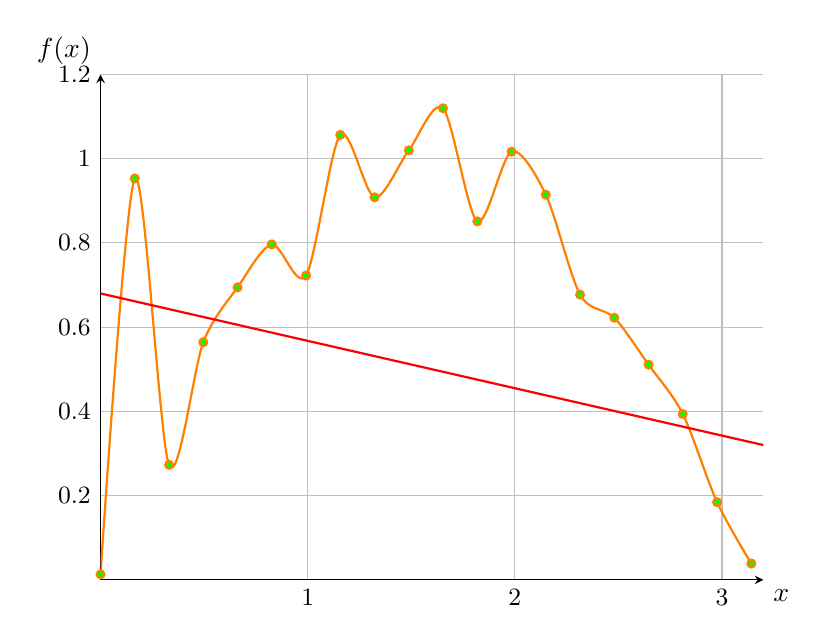
\begin{tikzpicture}
    \begin{axis}[
        axis lines=middle,
        xmin=0, xmax=3.2,
        ymin=0, ymax=1.2,
        xlabel={$x$},
        ylabel={$f(x)$},
        ylabel style={at={(0,1)}, anchor=north},
        ytick={0.2,0.4,0.6,0.8,1.0,1.2},
        xtick={1,2,3},
        every axis x label/.style={at={(current axis.right of origin)}, anchor=north west},
        every axis y label/.style={at={(current axis.above origin)}, anchor=south east},
        yticklabel style={anchor=east},
        xticklabel style={anchor=north},
        width=10cm,
        height=8cm,
        axis line style={-stealth},
        grid=major,
        black,
        tick style={color=white},
        major tick length=0pt,
        minor tick length=0pt,
        ticklabel style={font=\small}
    ]
    
    % Original data
    \addplot[
        color=orange,
        mark=*,
        mark options={scale=0.7, fill=green},
        thick,
        smooth
    ] coordinates {
        (0.0, 0.01313289) (0.16534698, 0.9531357) (0.33069396, 0.27303831) (0.49604095, 0.56426336) (0.66138793, 0.69446266) 
        (0.82673491, 0.79658221) (0.99208189, 0.72262249) (1.15742887, 1.0565153) (1.32277585, 0.90835232) (1.48812284, 1.01992807) 
        (1.65346982, 1.11962864) (1.8188168, 0.85117504) (1.98416378, 1.01662771) (2.14951076, 0.91446878) (2.31485774, 0.67722208) 
        (2.48020473, 0.6222458) (2.64555171, 0.511015) (2.81089869, 0.39366855) (2.97624567, 0.18442382) (3.14159265, 0.03879388)
    };
    
    % Regression line
    \addplot[
        color=red,
        thick
    ] coordinates {
        (0.0, 0.68) (3.2, 0.32)
    };
    
    % Customizations
    % \node[above] at (axis cs:2.5,1.15) {\huge $\boldsymbol{f(x)}$};
    
    \end{axis}
\end{tikzpicture}
\caption{مثالی از بیش‌برازش و کم‌برازش؛ خط قرمز مدل کم‌برازش شده است و خط زرد مدل بیش‌برازش شده}
\label{overfittingUnderfitting}
\end{figure}

\begin{center}
    \scalebox{1.2}{$\color{red} Error = 5.3$} \\
    \scalebox{1.2}{$\color{orange} Error = 0.0$}
\end{center}

\color{black}

به نظر می‌رسد که مدل زرد رنگ خطای بسیار کمتری دارد. اما آیا در واقعیت هم همین قضیه صدق می‌کند؟
برای این کار می‌توانیم بخشی از داده‌های خود را کنار گذاشته و برای تست مدل استفاده کنیم که در به رنگ آبی نمایش دادیم: 

\begin{figure}[!htp]
    \centering    
    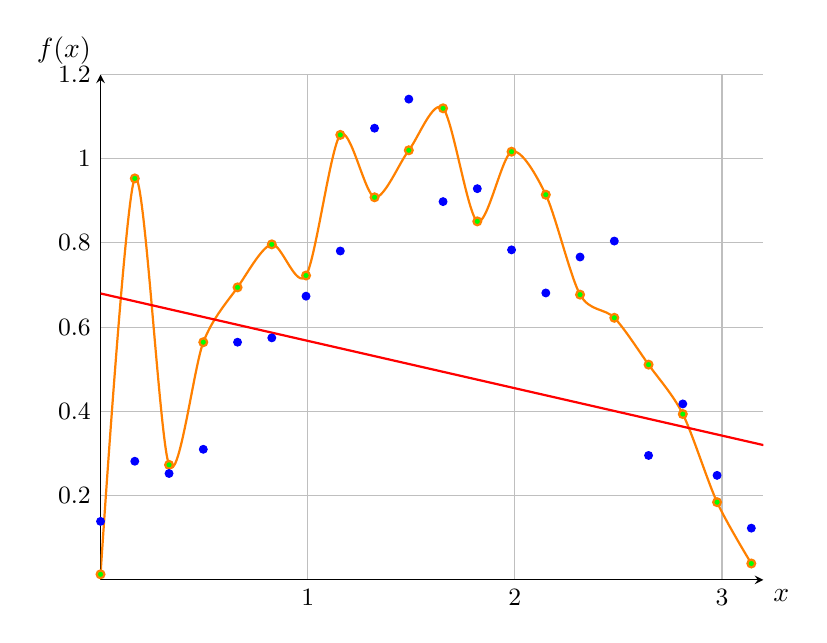
\begin{tikzpicture}
        \begin{axis}[
            axis lines=middle,
            xmin=0, xmax=3.2,
            ymin=0, ymax=1.2,
            xlabel={$x$},
            ylabel={$f(x)$},
            ylabel style={at={(0,1)}, anchor=north},
            ytick={0.2,0.4,0.6,0.8,1.0,1.2},
            xtick={1,2,3},
            every axis x label/.style={at={(current axis.right of origin)}, anchor=north west},
            every axis y label/.style={at={(current axis.above origin)}, anchor=south east},
            yticklabel style={anchor=east},
            xticklabel style={anchor=north},
            width=10cm,
            height=8cm,
            axis line style={-stealth},
            grid=major,
            black,
            tick style={
            smooth=white},
            major tick length=0pt,
            minor tick length=0pt,
            ticklabel style={font=\small}
        ]
        
        % Original data
        \addplot[
            color=orange,
            mark=*,
            mark options={scale=0.7, fill=green},
            thick,
            smooth
        ] coordinates {
            (0.0, 0.01313289) (0.16534698, 0.9531357) (0.33069396, 0.27303831) (0.49604095, 0.56426336) (0.66138793, 0.69446266) 
            (0.82673491, 0.79658221) (0.99208189, 0.72262249) (1.15742887, 1.0565153) (1.32277585, 0.90835232) (1.48812284, 1.01992807) 
            (1.65346982, 1.11962864) (1.8188168, 0.85117504) (1.98416378, 1.01662771) (2.14951076, 0.91446878) (2.31485774, 0.67722208) 
            (2.48020473, 0.6222458) (2.64555171, 0.511015) (2.81089869, 0.39366855) (2.97624567, 0.18442382) (3.14159265, 0.03879388)
        };

        \addplot[
            color=blue,
            mark=*,
            mark options={scale=0.7, fill=blue},
            only marks
        ] coordinates {
            (0.0, 0.13878516) (0.16534698, 0.28160998) (0.33069396, 0.25253683) (0.49604095, 0.30999755) (0.66138793, 0.56426281) (0.82673491, 0.5745891) (0.99208189, 0.67355963) (1.15742887, 0.78081114) (1.32277585, 1.07239615) (1.48812284, 1.14142923) (1.65346982, 0.89806727) (1.8188168, 0.92881436) (1.98416378, 0.78349175) (2.14951076, 0.68117417) (2.31485774, 0.76652376) (2.48020473, 0.80442836) (2.64555171, 0.29534375) (2.81089869, 0.41772831) (2.97624567, 0.24808496) (3.14159265, 0.12275737)
        };
        
        % Regression line
        \addplot[
            color=red,
            thick
        ] coordinates {
            (0.0, 0.68) (3.2, 0.32)
        };
        
        % Customizations
        % \node[above] at (axis cs:2.5,1.15) {\huge $\boldsymbol{f(x)}$};
        
        \end{axis}
    \end{tikzpicture}
    \caption{استفاده از داده‌های تست برای ارزیابی مدل}
    \label{overfittingUnderfitting}
    \end{figure}

    \begin{center}
        \scalebox{1.2}{$\color{red} Error_{train} = 5.3, Error_{test} = 5.6$} \\
        \scalebox{1.2}{$\color{orange} Error_{train} = 0.0, Error_{test} = 3.6$}
    \end{center}

\color{black}

همانظور که مشاهده می‌کنید، با وجود اینکه خطای مدل زرد در داده‌های آموزش ۰ می‌باشد، هنگامی که با داده‌هایی مواجه می‌شویم که مدل تا به حال آنها را ندیده، به یک بازه خطا به شدت افزایش پیدا می‌کند. این یعنی مدل داده‌های آموزش را "حفظ کرده" و "یاد نگرفته". اگر بخواهیم یک مثال ملموس‌تر بزنیم، می‌توانیم اینگونه فرض کنیم: تصور کنید که شما به شهر جدیدی رفته‌اید و نیاز به تاکسی پیدا می‌کنید. تاکسی از شما پول زیادی می‌گیرد و از آن پس فکر می‌کنید همه تاکسی‌های آن شهر همین رفتار را دارند؛ این می‌شود بیش برازش. در مقابل آن فرض کنید که حتی پس از ۲۰۰ بار سوار تاکسی شدن در شهر خودتان و زمانی که همه آن تاکسی‌ها پول زیاد و ناحقی از شما دریافت کردند هنوز هم یاد نگرفته‌اید که نباید در آن شهر از تاکسی استفاده کنید.

برای اینکه از بیش‌برازش جلوگیری کنیم نباید مدلمان بیش از حد پیچیده باشد و برای اینکه از کم‌برازش جلوگیری کنیم نباید مدلمان بسیار ساده. پیدا کردن مدل با پیچیدگی مناسب بستگی به نوع داده‌ها و مهارت شخص درحال طراحی مدل دارد. البته برای این کار ابزار‌هایی مانند \lr{Regularization} هم وجود دارد که از پیچیده شدن بیش‌از‌حد مدل اجتناب کند. به نظر می‌رسد برای این نوع داده‌ها تابعی درجه ۲ کافی باشد.

به نظر می‌رسد برای داده‌های ما یک مدل درجه ۲ می‌تواند نتیجه خوبی را بدهد:


\begin{figure}[!htp]
    \centering    
    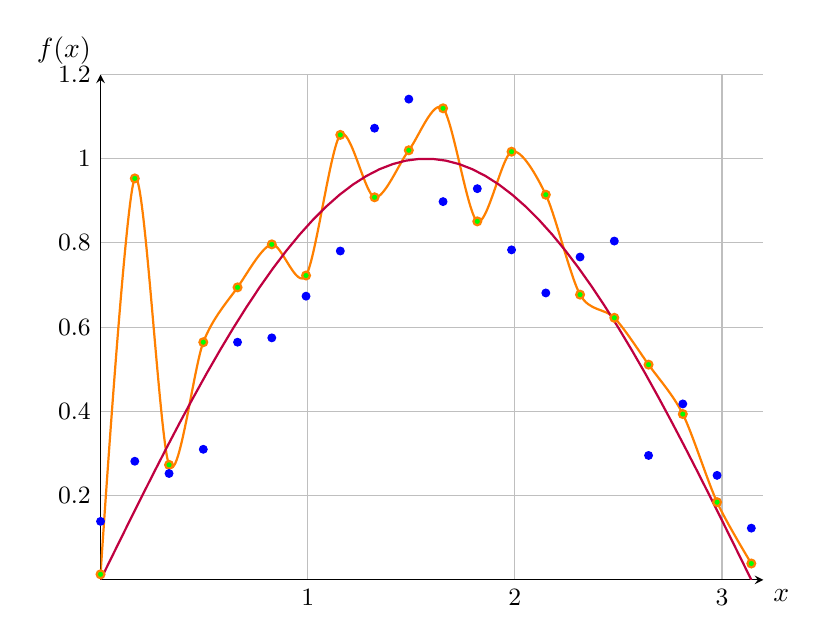
\begin{tikzpicture}
        \begin{axis}[
            axis lines=middle,
            xmin=0, xmax=3.2,
            ymin=0, ymax=1.2,
            xlabel={$x$},
            ylabel={$f(x)$},
            ylabel style={at={(0,1)}, anchor=north},
            ytick={0.2,0.4,0.6,0.8,1.0,1.2},
            xtick={1,2,3},
            every axis x label/.style={at={(current axis.right of origin)}, anchor=north west},
            every axis y label/.style={at={(current axis.above origin)}, anchor=south east},
            yticklabel style={anchor=east},
            xticklabel style={anchor=north},
            width=10cm,
            height=8cm,
            axis line style={-stealth},
            grid=major,
            black,
            tick style={
            smooth=white},
            major tick length=0pt,
            minor tick length=0pt,
            ticklabel style={font=\small}
        ]
        
        % Original data
        \addplot[
            color=orange,
            mark=*,
            mark options={scale=0.7, fill=green},
            thick,
            smooth
        ] coordinates {
            (0.0, 0.01313289) (0.16534698, 0.9531357) (0.33069396, 0.27303831) (0.49604095, 0.56426336) (0.66138793, 0.69446266) 
            (0.82673491, 0.79658221) (0.99208189, 0.72262249) (1.15742887, 1.0565153) (1.32277585, 0.90835232) (1.48812284, 1.01992807) 
            (1.65346982, 1.11962864) (1.8188168, 0.85117504) (1.98416378, 1.01662771) (2.14951076, 0.91446878) (2.31485774, 0.67722208) 
            (2.48020473, 0.6222458) (2.64555171, 0.511015) (2.81089869, 0.39366855) (2.97624567, 0.18442382) (3.14159265, 0.03879388)
        };

        \addplot[
            color=blue,
            mark=*,
            mark options={scale=0.7, fill=blue},
            only marks
        ] coordinates {
            (0.0, 0.13878516) (0.16534698, 0.28160998) (0.33069396, 0.25253683) (0.49604095, 0.30999755) (0.66138793, 0.56426281) (0.82673491, 0.5745891) (0.99208189, 0.67355963) (1.15742887, 0.78081114) (1.32277585, 1.07239615) (1.48812284, 1.14142923) (1.65346982, 0.89806727) (1.8188168, 0.92881436) (1.98416378, 0.78349175) (2.14951076, 0.68117417) (2.31485774, 0.76652376) (2.48020473, 0.80442836) (2.64555171, 0.29534375) (2.81089869, 0.41772831) (2.97624567, 0.24808496) (3.14159265, 0.12275737)
        };
        
        % Regression line
        \addplot[
            color=purple,
            thick
        ] coordinates {
            (0.0, 0.0) (0.0641141357875468, 0.06407021998071291) (0.1282282715750936, 0.127877161684506) (0.19234240736264038, 0.1911586287013723) (0.2564565431501872, 0.25365458390950735) (0.32057067893773394, 0.31510821802362066) (0.38468481472528077, 0.3752670048793741) (0.4487989505128276, 0.4338837391175581) (0.5129130863003744, 0.49071755200393785) (0.5770272220879211, 0.5455349012105486) (0.6411413578754679, 0.5981105304912159) (0.7052554936630148, 0.6482283953077884) (0.7693696294505615, 0.6956825506034864) (0.8334837652381083, 0.7402779970753155) (0.8975979010256552, 0.7818314824680298) (0.9617120368132019, 0.8201722545969559) (1.0258261726007487, 0.8551427630053461) (1.0899403083882955, 0.886599306373) (1.1540544441758422, 0.9144126230158124) (1.218168579963389, 0.9384684220497603) (1.2822827157509358, 0.9586678530366606) (1.3463968515384828, 0.9749279121818236) (1.4105109873260295, 0.9871817834144501) (1.4746251231135763, 0.9953791129491982) (1.538739258901123, 0.9994862162006879) (1.6028533946886698, 0.9994862162006879) (1.6669675304762166, 0.9953791129491982) (1.7310816662637634, 0.9871817834144502) (1.7951958020513104, 0.9749279121818236) (1.8593099378388571, 0.9586678530366607) (1.9234240736264039, 0.9384684220497604) (1.9875382094139507, 0.9144126230158125) (2.0516523452014974, 0.8865993063730001) (2.1157664809890444, 0.8551427630053462) (2.179880616776591, 0.8201722545969561) (2.243994752564138, 0.7818314824680299) (2.3081088883516845, 0.7402779970753157) (2.3722230241392315, 0.6956825506034865) (2.436337159926778, 0.6482283953077888) (2.500451295714325, 0.5981105304912161) (2.5645654315018716, 0.545534901210549) (2.6286795672894185, 0.49071755200393813) (2.6927937030769655, 0.43388373911755823) (2.756907838864512, 0.3752670048793745) (2.821021974652059, 0.3151082180236209) (2.8851361104396056, 0.2536545839095078) (2.9492502462271526, 0.19115862870137254) (3.013364382014699, 0.1278771616845065) (3.077478517802246, 0.06407021998071323) (3.141592653589793, 1.2246467991473532e-16)
        };
        
        % Customizations
        % \node[above] at (axis cs:2.5,1.15) {\huge $\boldsymbol{f(x)}$};
        
        \end{axis}
    \end{tikzpicture}
    \caption{مدل مناسب}
    \label{overfittingUnderfitting}
    \end{figure}

    \begin{center}
        \scalebox{1.2}{$\color{red} Error_{train} = 5.3, Error_{test} = 5.6$} \\
        \scalebox{1.2}{$\color{orange} Error_{train} = 0.0, Error_{test} = 3.6$} \\
        \scalebox{1.2}{$\color{purple} Error_{train} = 2.2, Error_{test} = 2.8$}
    \end{center}

\color{black}

همانطور که مشاهده می‌کنید، با وجود اینکه خطای مدل بنفش برای داده‌های آموزش ۲.۲ می‌باشد. برای داده‌های آزمون خطای این مدل از هر دو مدل بیش‌برازش شده و کم‌برازش شده، کمتر است.

\subsection{نقاط پرت (\lr{Outliers})}
به اشکال خاصی از داده‌ها اطلاق می‌شود که از الگوهای عمومی یا میانگین معمول داده‌ها بیرون می‌افتند. به عبارت دیگر، این داده‌ها به دلایلی مثل خطای اندازه‌گیری یا وقوع رویدادهای نادر (از جمله خطا یا اطلاعات اشتباه) از سایر نمونه‌ها متمایز می‌شوند. این اشکال داده‌ها می‌توانند تحلیل‌های آماری را تحت تأثیر قرار داده و به تصمیمات نادرستی منجر شوند. بنابراین، شناسایی و مدیریت \lr{outliers} در تحلیل داده‌ها از اهمیت بسیاری برخوردار است.
یکی دیگر از دلایل دیگر به وجود آمدن \lr{outlier}ها می‌تواند این باشد که ما ابعاد دیگر داده را درنظر نگرفتیم. مثلا برای قیمت خانه‌ها تنها فاکتور مشخص کننده قیمت خانه متراژ آن نیست، بلکه فاکتور‌های دیگر از جمله موقعیت مکانی، امکانات دیگر خانه و غیره در این تصمیم‌گیری نقش دارند. بدون داشتن ابعاد دیگر داده نمی‌توانیم تشخیص دهیم که دلیل به وجود آمدن آن‌ها چه چیزیست.

در شکل زیر دور یکی از \lr{outlier}ها خط کشیده شده است.


\begin{figure}[!htp]
    \centering
    \begin{tikzpicture}
    \begin{axis}[
        xlabel={\lr{$m^2$} خانه متراژ},
        ylabel={\lr{\$} خانه قیمت},
        grid=major,
        width=10cm,
        height=10cm,
        axis lines=middle,
        scatter/classes={
            a={mark=*,blue},
            b={mark=*,red}
        }
    ]
    
    % Scatter plot points
    \addplot[scatter,only marks,scatter src=explicit symbolic]
    table[meta=label] {
        x y label
        193.75 326250.0 a
        93.75 93000.0 a
        175.0 210000.0 a
        50.0 37500.0 a
        343.75 450000.0 a
        437.5 412500.0 a
        412.5 439500.0 a
        293.75 247500.0 a
        143.75 300000.0 a
        481.25 435000.0 a
        312.5 495000.0 a
        75.0 90000.0 a
        368.75 270000.0 a
        475.5 105000.0 a
        450.0 450000.0 a
        85.3 150000.0 a
    };
    
    % Regression line
    \addplot[
        domain=0:500, 
        samples=100, 
        color=red,
        thick
    ]{653.7*x + 102522.4};
    
    \draw[green,-latex, very thick](axis cs: 420,105000) -- (axis cs: 475, 105000);

    \end{axis}
    \end{tikzpicture}
    \caption{نمایش یک نقطه پرت}
    \label{HousePrices}
    \end{figure}
    

\clearpage
\section{دسته‌ بندی}
\subsection{مقدمه}

اکنون وارد مبحث \lr{Classification} (دسته بندی) میشوم. در \lr{Supervised Classification} هدف ما یادگیری تابع‌ای است که بتواند ورودی را به گروه‌های گسسته دسته بندی کند.

\subsection{انواع دسته‌ بندی}
\subsubsection{دسته‌ بندی دودوی}
در ابتدا بهتر است که به انواع مختلف \lr{Classification} اشاره کنیم. ساده ترین نوع \lr{Binary Classification} است که در آن بودن و یا نبودن مورد بررسی قرار میگیرند و ورودی حداکثر دو نوع دسته خروجی دارد.
\begin{figure}[H]
    \center
    \begin{minipage}[b]{0.4\textwidth}
        \center
        \includegraphics[width=\textwidth, height=6cm, width=4.5cm]{Classification-img1.png}
        \label{Classification-img1}
    \end{minipage}
    \hfill
    \begin{minipage}[b]{0.5\textwidth}
        \center
        \includegraphics[width=\textwidth, height=6.5cm]{Classification-img2.png}
        \label{Classification-img2}
    \end{minipage}
    \caption{\lr{Binary Classification.}}
\end{figure}

\subsubsection{دسته‌ بندی چند کلاسه}
نوع دوم \lr{MultiClass Classification} است که در آن تعداد دسته‌های که ورودی میتواند در آنها قرار گیرد بیشتر از 2 است.

\begin{figure}[H]
    \center
    \begin{minipage}[b]{0.4\textwidth}
        \center
        \includegraphics[width=\textwidth, height=6cm, width=6cm]{Classification-img3.png}
        \label{Classification-img3}
    \end{minipage}
    \hfill
    \begin{minipage}[b]{0.5\textwidth}
        \center
        \includegraphics[width=\textwidth, height=6.5cm]{Classification-img4.png}
        \label{Classification-img4}
    \end{minipage}
    \caption{\lr{MultiClass Classification.}}
\end{figure}

\clearpage
مسائل \lr{MultiClass Classification} به یکی از دو صورت زیر مدل سازی میشوند:

یک در مقابل همه (باقی): در این روش مسئله را به چند زیر مسئله کوچک تر تبدیل میکنیم، به این صورت که هر زیر مسئله خود یک مسئله \lr{Binary Classification} است و در آن عضویت هر ورودی برای هر دسته در مقابل سایر دسته‌ها بررسی میشود.

\begin{figure}[H]
    \center
    \includegraphics[height=8cm]{Classification-img5.png}
    \label{Classification-img5}
    \caption{\lr{MultiClass Classification.}}
\end{figure}

یک در مقابل یک: در این روش نیز مسئله را به چند زیر مسئله کوچک تر تبدیل میکنیم، به این صورت که هر زیر مسئله خود یک مسئله \lr{Binary Classification} است و در آن مانند مثال زیر برای سه دسته مسئله به سه مسئله \lr{Binary Classification} تقسیم بندی میشود و ورودی را با هر سه مدل ایجاد شده بررسی میکنیم.

\begin{figure}[H]
    \center
    \includegraphics[height=8cm]{Classification-img6.png}
    \label{Classification-img6}
    \caption{\lr{MultiClass Classification.}}
\end{figure}

\clearpage
\subsubsection{دسته‌ بندی چند دسته‌ای}

آخرین دسته از مسائل \lr{Classification} مسائل \lr{Multilable Classification} هستند که مشابه با مسائل \lr{MultiClass Classification} میباشند با این تفوت که هر ورودی میتواند به بیش از یک دسته تعلق داشته باشد.

\begin{figure}[H]
    \center
    \includegraphics[height=8cm]{Classification-img7.png}
    \label{Classification-img7}
    \caption{\lr{Multilable Classification.}}
\end{figure}

\subsection{نگاهی عمیق تر به دسته‌ بندی دودوی}

در اینجا به دلیل ذات آسان‌تر مسائل \lr{Binary Classification} و زمان محدود ارائه تمرکز خود را بر روی مسائل \lr{Binary Classification} می‌گذاریم.
نمونه‌های از مسائل \lr{Binary Classification} مانند تشخیص اسکناس‌های اصلی از تقلبی و یا تشخیص روزهای بارانی و غیر بارانی هستند.

\begin{figure}[H]
    \center
    \begin{minipage}[b]{0.45\textwidth}
        \center
        \includegraphics[width=\textwidth, height=7cm, width=7cm]{Classification-img9.png}
        \label{Classification-img9}
    \end{minipage}
    \hfill
    \begin{minipage}[b]{0.45\textwidth}
        \center
        \includegraphics[width=\textwidth, height=7cm, width=7cm]{Classification-img8.png}
        \label{Classification-img8}
    \end{minipage}
    \caption{\lr{Binary Classification.}}
\end{figure}

\clearpage
در نظر بگیرید که برای برای حل مسائل روز‌های بارانی به روش \lr{Supervised Classification} یک جدول از روز‌های گذشته داریم که در آن برای هر روز میزان رطوبت، فشار هوا و بارانی بودن و نبودن آن روز ثبت شده اند.


\begin{table}[H]
    \centering
    \scalebox{1.2}{\begin{tabular}{cccc}
        \lr{Rain} & \lr{Pressure} & \lr{Humidity} & \lr{Date} \\
        \lr{Rain} & \lr{999.7}  & \lr{93\%} & \lr{January 1} \\
        \lr{No Rain} & \lr{1015.5}  & \lr{49\%}  & \lr{January 2} \\
        \lr{No Rain} & \lr{10.31.1}  & \lr{79\%}  & \lr{January 3} \\
        \lr{Rain} & \lr{984.9}  & \lr{65\%}  & \lr{January 4} \\
        \lr{Rain} & \lr{975.2}  & \lr{90\%}  & \lr{January 5} \\
    \end{tabular}}
    \caption{\lr{Rainy days}}
    \label{tab:Rainy-days}
\end{table}

در طبیعت یک تابع وجود دارد که به صورت زیر کار میکند:

\begin{equation}
    \scalebox{1.2}{${f(humidity,\:pressure) = Rain \; or \; Not \; Rain}$}
    \label{f-function}
\end{equation}

این تابع با دریافت رطوبت و فشار هوا برای هر روز مشخص میکند که آیا آن روز باید باران ببارد یا خیر.(در واقعیت عوامل بسیار بیشتر و پیچیده‌تری در تایین وضعیت آب‌وهوا دخیل هستند اما به دلیل جلوگیری از پیچیده شدن بیش از حد از آنها صرف نظر میکنیم) از آنجا که این تابع نامشخص است هدف ما در اینجا رسیدن به تابعی \lr{heuristic} (تقریبی) است که تا حد امکان مشابه به تابع اصلی در طبیعت باشد و امکان تشخیص روز‌های بارانی و غیربارانی را با دقت قابل توجهی فراهم کند.

\begin{equation}
    \scalebox{1.2}{${h(humidity,\:pressure) = Rain \; or \; Not \; Rain}$}
    \label{h-function}
\end{equation}

بهتر است داده‌های فرضی یک جدول رطوبت و فشار هوا را برای روز‌های بارانی و غیربارانی در یک محور مختصات بر اساس رطوبت و فشار هوا مانند زیر ترسیم کنیم:

\begin{figure}[H]
    \center
    \includegraphics[height=5cm]{Classification-img10.png}
    \label{Classification-img10}
    \caption{\lr{Binary Classification.}}
\end{figure}

در این شکل نقاط آبی نشان دهنده روز های بارانی و نقاط قرمز نشان‌دهنده روز‌های غیربارانی هستند. اگر فردی تصویر زیر را به شما نشان دهد و از شما بخواهد که حدس خود را درباره رنگ نقطه سفید بیان کنید (تخمین بزنید که این روز بارانی است یا خیر) چه پاسخی میدهید؟

\begin{figure}[H]
    \center
    \includegraphics[height=5cm]{Classification-img11.png}
    \label{Classification-img11}
    \caption{\lr{Binary Classification.}}
\end{figure}

تقریبا حدس تمامی افراد (عاقل) به این صورت خواهد بود که رنگ حقیقی این نقطه آبی است زیرا در میان نقاط آبی محاصره شده است. اگر حدس خود را بر اساس این منطق و این نکته که نزدیک ترین نقطه به سفید خود رنگ آبی دارد، منطق شما مشابه با تکنیک دسته‌بندی نزدیک‌ترین همسایه خواهد بود. در دسته‌بندی نزدیک‌ترین همسایه، در ابتدا نزدیک‌ترین نقطه به نقطه مورد سوال را یافته و به این گونه در نظر میگیریم که از آنجا که تمامی ویژگی‌های مستقل این دو نقطه مشابه هم هستند به احتمال فراوان ویژگی غیر وابسته آنان نیز (رنگ) یکسان خواهد بود.

\begin{figure}[H]
    \center
    \includegraphics[height=5cm]{Classification-img12.png}
    \label{Classification-img12}
    \caption{\lr{Binary Classification.}}
\end{figure}

حال مثال زیر را در نظر بگیرید:

\begin{figure}[H]
    \center
    \includegraphics[height=5cm]{Classification-img13.png}
    \label{Classification-img13}
    \caption{\lr{Binary Classification.}}
\end{figure}

اکنون چه حدسی برای نقطه سفید دارید؟ اگر بر اساس اصل نزدیک‌ترین همسایه پیش برویم انتظار میرود که رنگ این نقطه قرمز باشد (غیر بارانی).

\begin{figure}[H]
    \center
    \includegraphics[height=5cm]{Classification-img14.png}
    \label{Classification-img14}
    \caption{\lr{Binary Classification.}}
\end{figure}

اما همانطور که مشاهده میکنید در اطراف این نقطه تعداد بسیار بیشتری نقاط آبی قرار دارند و نقطه قرمز که نزدیک ترین نقطه به نقطه مورد نظر ما است یک داده \lr{outlier} است، بر همین اساس انتظار میرود که احتمال اینکه رنگ نقطه مورد نظر آبی باشد بیشتر است (هرچند نمیتوان با قاطعیت بیان کرد).

به منظور جلوگیری از بروز چنین موارد الگوریتم نزدیک‌ترین همسایه را کمی تغیر میدهیم، به این صورت که دیگر تنها بر اساس نزدیک ترین همسایه به نقطه مجهول تصمیم‌گیری نمیکنیم بلکه تعداد بیشتری از نقاط همسایه نزدیک را در نظر میگیرم و در میان آنها رای گیری میکنیم (به این منظور برای جلو گیری از برابر شدن تعداد آرا تعداد نقاط همسایه مورد بررسی را یک عدد فرد قرار میدهیم). روش بیان شده یک نسخه از الگوریتم نزدیک‌ترین همسایه است که \lr{k} نزدیک‌ترین همسایه نام دارد (\lr{k} تعداد همسایه‌های مورد بررسی است).

\begin{figure}[H]
    \center
    \includegraphics[height=7cm]{Classification-img15.png}
    \label{Classification-img15}
    \caption{\lr{Binary Classification.}}
\end{figure}

\begin{figure}[H]
    \center
    \includegraphics[height=5cm]{Classification-img16.png}
    \label{Classification-img16}
    \caption{\lr{Binary Classification.}}
\end{figure}

\clearpage
الگوریتم \lr{k} نزدیک‌ترین همسایه به دلیل آسانی استفاده‌های زیادی دارد اما به دلیل مشکلاتی نظیر اینکه برای به دست آوردن نزدیک ترین نقاط هماسیه به نقطه مجهول لازم است فاصله نقطه مجهول با تمامی نقاط را محاسبه کنیم کاراری و عملکرد الگوریتم در دیتاست‌های بسیار بزرگ به شدت کاهش میابد. به این دلیل اکنون روش دیگری را برای حل مسائل \lr{Binary Classification} بیان میکنیم. مثال زیر را در نظر بگیرد.

\begin{figure}[H]
    \center
    \includegraphics[height=5cm]{Classification-img17.png}
    \label{Classification-img17}
    \caption{\lr{Binary Classification.}}
\end{figure}

آیا به نظر شما میتوان این نقاط را به وسیله یک خط مرزی از هم جدا کرد؟ پاسخ به این سوال مثبت است. میتوان مانند تصویر زیر عمل کرد.

\begin{figure}[H]
    \center
    \includegraphics[height=5cm]{Classification-img18.png}
    \label{Classification-img18}
    \caption{\lr{Binary Classification.}}
\end{figure}

در واقعیت داده‌های ما به این صورت تمیز و خطی جداپزیر \lr{(linearly separable)} نیستند.   

\begin{figure}[H]
    \center
    \includegraphics[height=5cm]{Classification-img19.png}
    \label{Classification-img19}
    \caption{\lr{Binary Classification.}}
\end{figure}

\clearpage
هدف ما این است که خطی را به دست آوریم که به بهترین شکل ممکن داده را از هم جدا کند (در آینده در رابطه با نحوه ارزیابی خطوط مختلف بحث خواهیم کرد). به منظور رسیدن به این هدف میتوان به این صورت تصور کرد که ما میخواهیم یک تابع \lr{heuristic} را به گونه‌ای به دست آوریم که که مانند شکل زیر با دریافت مقادیر برای هر ورودی، مشخص کند که آن ورودی یک روز بارانی است یا خیر.

\begin{equation}
    \scalebox{1.2}{${x_{1} = Humidity}$}
    \label{x1Humidity}
\end{equation}

\begin{equation}
    \scalebox{1.2}{${x_{2} = Pressure}$}
    \label{x2Pressure}
\end{equation}

\begin{equation}
    \scalebox{1.2}{${h(x\textsubscript{\lr{1}},\:x\textsubscript{\lr{2}}) = Rain \; if \; w\textsubscript{\lr{0}} \; + \; w\textsubscript{\lr{1}}x\textsubscript{\lr{1}} \; + \; w\textsubscript{\lr{1}}x\textsubscript{\lr{2}} \; \ge \; 0 \; otherwise \; No \; Rain}$} \label{h-function-2}
\end{equation}

در این تابع \lr{w} ها وزن \lr{(wight)} نام دارند. آنها را به صورت یک \lr{vector} مینویسیم و ورودی را نیز به حالت \lr{vector} در میآوریم (به \lr{vector} ورودی مقدار یک را به عنوان ضریب برای \lr{w\textsubscript{0}} اضافه میکنیم تا اندازه \lr{vector} ورودی با اندازه \lr{vector} وزن‌ها یکسان باشد و بتوانیم \lr{dot product} آنها را محاسبه کنیم). 

\begin{equation}
    \scalebox{1.2}{${Weight \; Vector \; w : (w\textsubscript{\lr{0}},\:w\textsubscript{\lr{1}},\:w\textsubscript{\lr{2}})}$}
    \label{Weights}
\end{equation}

\begin{equation}
    \scalebox{1.2}{${Input \; Vector \; x : (1,\:x\textsubscript{\lr{1}},\:w\textsubscript{\lr{2}})
    \label{inputs}}$}
\end{equation}

\begin{equation}
    \scalebox{1.2}{${w . x : w\textsubscript{\lr{0}} + :w\textsubscript{\lr{1}}x\textsubscript{\lr{1}}+ :w\textsubscript{\lr{2}}x\textsubscript{\lr{2}}}$}
    \label{wdotx}
\end{equation}

\begin{equation}
    \scalebox{1.2}{${h\textsubscript{\lr{w}}(x) = 1 \; if \; w \; . \; x \; \>= \; 0 \; otherwise \; 0}$}
    \label{h-function-3}
\end{equation}

حال به نحوه چگونگی مقادیر وزن‌ها میرسیم. برای محاسبه مقادیر وزن‌ها میتوانیم به صورت زیر عمل کنیم. هربار برای هر ورودی مقدار تابع را محاسبه میکنیم، اگر هردو یکسان بودند تغیری در وزن‌ها ایجاد نمیشود، اما اگر متفاوت بودند بنا بر میزان تفاوت \lr{(alpha (learning rate))} مقادیر وزن‌های جدید را محاسبه میکنیم.

\begin{center}
    \scalebox{1.2}{\lr{Perceptron Learning Rule}}
    
    \scalebox{1.2}{\lr{Given data point (x, y), update each weight according to:}}
    
    \begin{equation}
        \scalebox{1.2}{${w\textsubscript{\lr{i}} = w\textsubscript{\lr{i}} + \alpha(y - h\textsubscript{\lr{w}}(x)) \times x\textsubscript{\lr{i}}}$}
        \label{w-update-1}
    \end{equation}
    \begin{equation}
        \scalebox{1.2}{${w\textsubscript{\lr{i}} = w\textsubscript{\lr{i}} + \alpha(actual\;value - estimate) \times x\textsubscript{\lr{i}}}$}
        \label{w-update-2}
    \end{equation}
\end{center}

\clearpage
اگر از این روش پیروی کنیم به یک تابع فعال کننده مانند شکل زیر میرسیم.

\begin{figure}[H]
    \center
    \includegraphics[height=5cm]{Classification-img20.png}
    \label{Classification-img20}
    \caption{\lr{Binary Classification.}}
\end{figure}

در این تابع اگر مقدار ضرب \lr{vector} های \lr{w} و \lr{x} (بر اساس مقدار ورودی \lr{x}) از یک مقدار مشخصی کمتر باشد تابع آن ورودی را به عنوان روز غیر بارانی و اگر مقدار ضرب \lr{vector} های \lr{w} و \lr{x} بیشتر از آن مقدار باشد آن ورودی را به عنوان یک روز بارانی در نظر میگیرد.

به تصویر زیر دقت کنید.

\begin{figure}[H]
    \center
    \includegraphics[height=5cm]{Classification-img21.png}
    \label{Classification-img21}
    \caption{\lr{Binary Classification.}}
\end{figure}

این مدل هر دو ورودی سفید رنگ را به عنوان نقاط بارانی در نظر میگیرد. اما با توجه بیشتر به تصویر مشاهده میکنید که میزان دقتی که برای تعیین دسته این دو ورودی وجود دارد دارای تفاوت فاهشی است و نقطه سفید رنگ در سمت چپ پایین صفحه میتواند در واقعیت یک روز غیر بارانی باشد. این نوع تابع \lr{hard threshold} این امکان را به ما نمیدهد که میزان اطمینان مدل از گروه تعیین شده برای ورودی را به دست آوریم و به همین منظور اغلب از تابع \lr{logistic regression} که این امکان را به ما میدهد استفاده میکنیم.

\begin{figure}[H]
    \center
    \includegraphics[height=5cm]{Classification-img22.png}
    \label{Classification-img22}
    \caption{\lr{Binary Classification.}}
\end{figure}

\clearpage
\subsection{ارزیابی مدل}
برای ارزیابی مدل میتوان از روش‌های متنوعی استفاده کرد که در اینجا یکی از آنها را بیان میکنیم. ارزیابی مدل‌های دسته‌بندی را میتوان با روشی به نام \lr{0-1 loss} انجام داد، به این صورت که تعداد داده‌های که به اشتباه دسته بندی شده‌اند را محاسبه کرده و هدف خود را کمینه کردن مقدار این تابع قرار میدهیم.

\begin{figure}[H]
    \center
    \includegraphics[height=5cm]{Classification-img23.png}
    \label{Classification-img23}
    \caption{\lr{Binary Classification.}}
\end{figure}


\clearpage
\begin{thebibliography}{9}
\bibitem{misc}
\href{https://cs50.harvard.edu/ai/2024/}{\lr{CS50's Introduction to Artificial Intelligence with Python}}

\bibitem{misc}
\href{https://youtu.be/-g0iJjnO2_w?si=DVcD4dhUWdf8uKGn}{\lr{Learning - Lecture 4 - CS50's Introduction to Artificial Intelligence with Python 2020}}

\bibitem{misc}
\href{https://en.wikipedia.org/wiki/Machine_learning}{\lr{Machine learning - Wikipedia}}

\bibitem{misc}
\href{https://en.wikipedia.org/wiki/Regression_analysis}{\lr{Regression analysis - Wikipedia}}

\bibitem{misc}
\href{https://en.wikipedia.org/wiki/Linear_regression}{\lr{Linear regression - Wikipedia}}

\bibitem{misc}
\href{https://youtu.be/R9OHn5ZF4Uo?si=PlffV1QOnI8nuaWO}{\lr{How AIs, like ChatGPT, Learn}}

\bibitem{misc}
\href{https://mlu-explain.github.io/linear-regression/}{\lr{Linear Regression; A Visual Introduction To (Almost) Everything You Should Know}}


\end{thebibliography}

\end{document}
